%------------------------------------------------------------------------------
\chapter*{Acknowledgements}
\label{sec:ack}
%------------------------------------------------------------------------------
When I was in eighth grade, I was asked what I wanted to be when I grow up. I said I wanted to be an astronomer. This was immediately followed by a second question, ah, So you want to go to space ? I said No, I want to look at it. In the end it turned out that I did a little bit of both. I went to Germany which was outer space for me and I looked at stars via an experiment in Argentina. This thesis is a result of that journey.

It took a village to raise this thesis. A crowded one at that with teachers family and friends without whom this would not have been possible.

The first people to thank are the teachers I have had during my time working on this thesis. It took me a few years to realize how lucky I was to be given an opportunity to write this thesis under the tutelage of Prof. Dr. Karl-Heinz Kampert. The way Prof. Kampert lets PhD students operate on their own terms is something that made my time here enjoyable and his group a perfect fit. He has been a constant source of inspiration and motivation. To have him in your corner backing you up be it regarding the content of this thesis or calling the mayor of Wuppertal to make sure I am not kicked out of the country (true story) made all the difference. 

I would also like to thank Prof. Dr. Jaime Alvarez Muñiz for agreeing to be my second de facto supervisor. His guidance and support has been invaluable. While sitting in his office in Santiago de Compostela, he has always been an email and Zoom call away answering my repeated questions anytime. Thank you, I could not have asked for more. Like I said to you, I am yet to get the time and opportunity to complete my Camino to your office, but I am sure I will get there soon. 

I have been blessed with even more great teachers who I need to thank. Dr. Julian Rautenberg, who I might have talked to for countless hours (always in five minute intervals) about the most trivial of things be it life or work. He always has a smile on his face and a solution to every problem or should I say challenge. Dr. Christian Pauli for being my next door office neighbour, who I bugged regarding the lab exercises all these years. Prof. Dr. Klaus Helbing for just being a fellow Bonner reminding me of my first home in Germany. Others in the Pierre Auger Collaboration like Prof. Dr. Enrique Zas, Prof. Dr. Piera Ghia and Prof. Dr. Alan Watson who have might not have been directly involved in this thesis but with their pertinent questions and supportive statements in some way helped me during the journey.

The second are my family. If a 15-year-old boy who left his home was not spared at the border during the partition of India, I would not have been here. My grandfather, Shanti Sarup Sehgal, who was my biggest supporter has shaped my life in multiple ways. He inculcated two things in me, the desire to succeed and to have fun while doing it. My grandmother Kusum Sehgal, who our family lost way too early but her spirit and memory lives on. Both of you continue to inspire me. My parents, Ravi and Rajni Sehgal, thank you for teaching me the value of hard work and sacrifice. You both cut short your dreams to make sure me and my brother could chase ours, I hope I can honour it. Without your constant support and sacrifices, I would not have been able to come to Germany and write this thesis. Thanks to my brother Sambhav for always providing me with the much-needed sports related distractions that kept me sane. 

I have a big family who have always checked up on my well-being and have been a constant source of support. Thank you Binu and Renu bua for always being there for me. Thank you Indu masi, Neeru masi and Vipin mama for always checking up on me. A big thanks to all my aunts and uncles.
In India the first cousins are like siblings and I have been lucky to have a bunch of them. Thank you to all of them, Ashish Bhaiya, Rinki bhaji, Divya di, Ankita di, Suhina di, Sadhika, Kartik, Jeevanshu , Chesta and Vanya for always making those short escapes to India my favourite times of the year. A special thanks to Kritika di or Dr. Kritika Khanna, you gave me one of the most valuable advice I have ever received, to not do the PhD if I just wanted the doctor title, but to do it if I wanted to learn something new. I hope I have done justice to that advice.     

My family now also includes my girlfriend Lélia Nagel. I am glad that I met you right before I started my thesis. Having a real doctor by my side who has dedicated her life to help others constantly grounds me. You have been a constant source of support and motivation. You have been my rock and my biggest cheerleader. Thank you for always being there for me and for making me a better person. I cannot wait to spend more time with you and make more memories.

Lastly, I have been blessed with a wonderful set of friends who have been my family away from home. Thank you to Svenja for being my best friend through the seven years I have been in Germany. We might not live in the same city any more, but you are always just a phone call away. Thank you to Prakhar, Lex, Rieka, Jan and Naseem for always keeping tabs on me and making sure I am doing fine. Starting this thesis during the pandemic was not easy but having the best roommates in the world in Steve and Fiona made it a lot of fun. A simple hi in the kitchen or a beer in the garden was all I needed to keep going. 

A special thanks to Dr. Jannis Pawlowsky, Dr. Leonel Morejon and Fabian Becker for helping with the editing of this thesis. Thank you to Michael Schimp for always answering my various questions and solving my problems without which this thesis would have never been completed. A big thanks to the whole Astroteilchen group for the academic and moral support and all the laughs we have shared. 

\begin{figure}[h!]
    \centering
    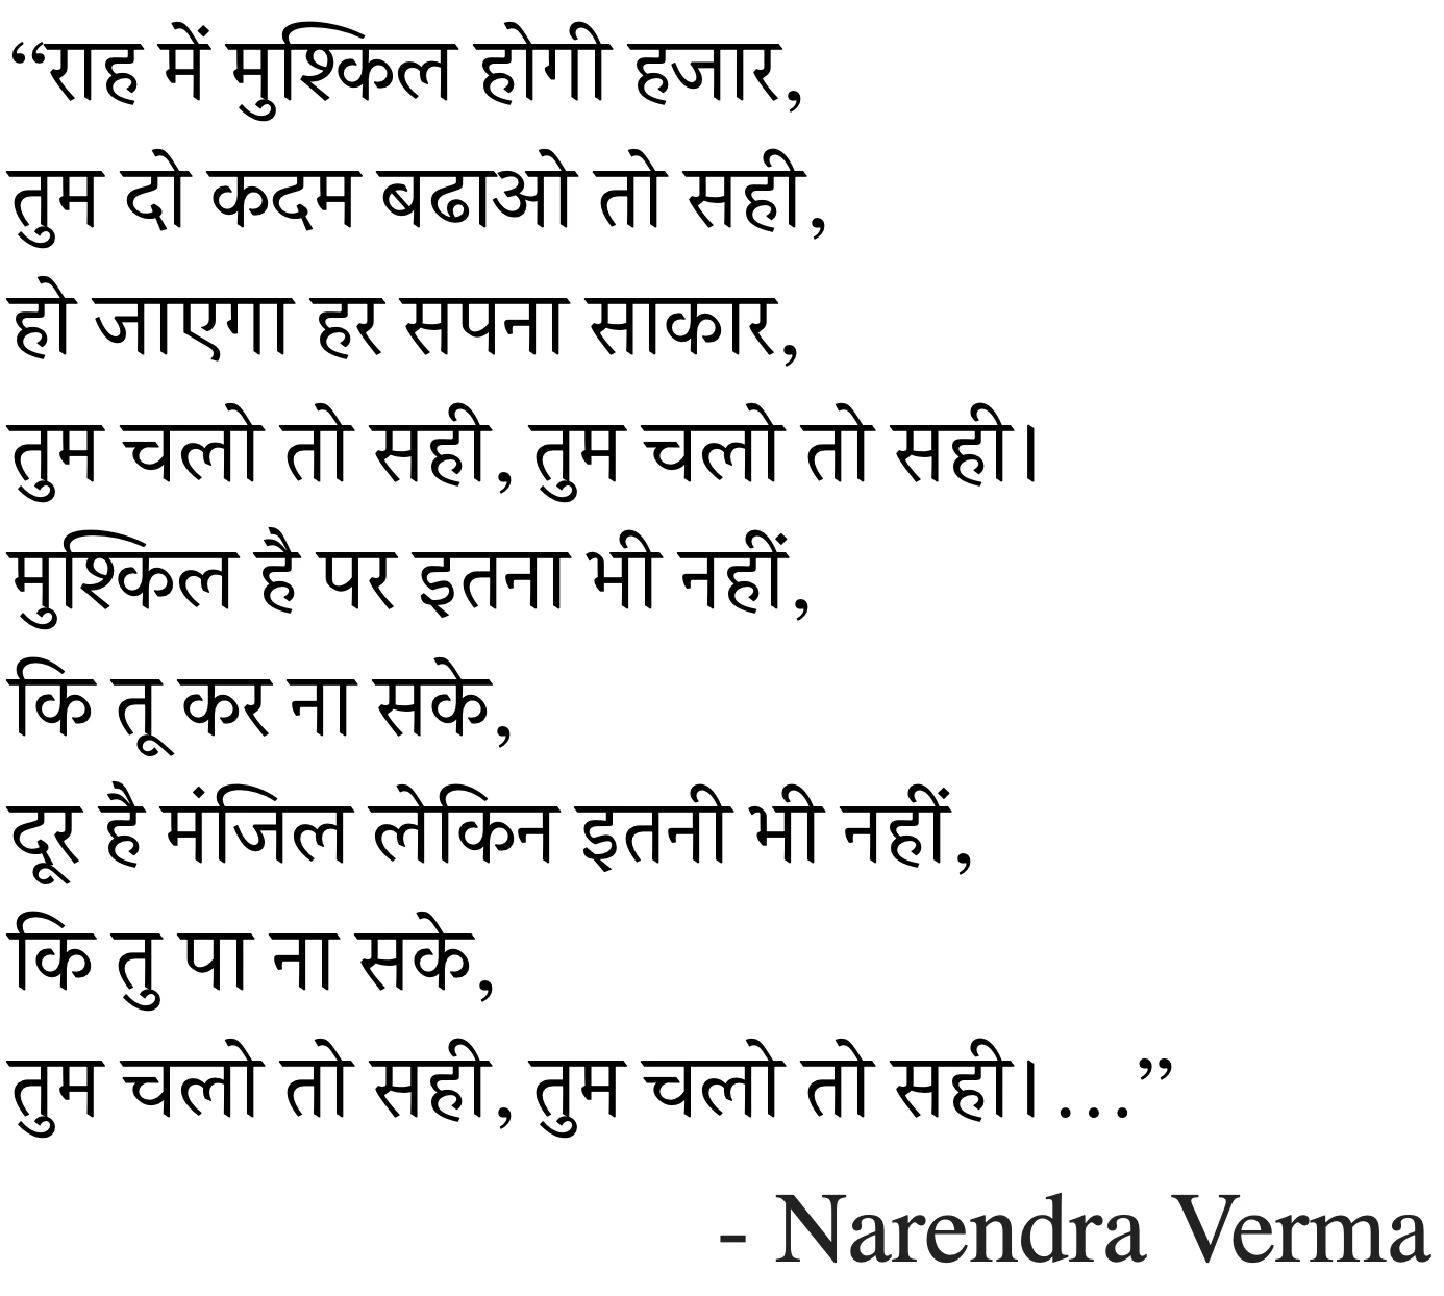
\includegraphics[width=0.65\textwidth]{thesis_figures/Poem_acknowledge.pdf}
    \caption*{}
  \end{figure}

%%% Local Variables:
%%% mode: latex
%%% TeX-master: "../mythesis"
%%% End:
